\documentclass[tikz,border=7pt]{standalone}
\usepackage{amsmath,amssymb}
\usetikzlibrary{arrows.meta,positioning}
\tikzset{vertex/.style={circle,draw,fill=cyan!12,minimum size=7mm,inner sep=1pt},box/.style={draw,rounded corners,fill=cyan!8,align=center,minimum height=12mm,minimum width=27mm}}
\begin{document}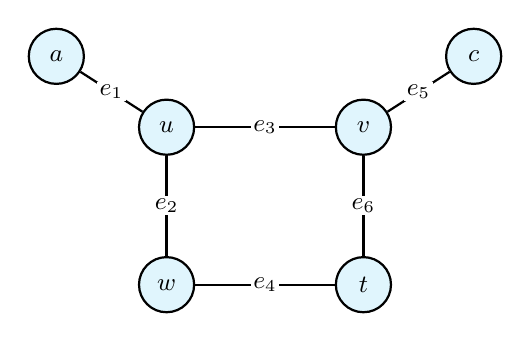
\begin{tikzpicture}[line width=0.8pt,font=\small]
\node[vertex] (va) at (-1.4,1.9) {$a$};
\node[vertex] (vu) at (0,1) {$u$};
\node[vertex] (vw) at (0,-1) {$w$};
\node[vertex] (vt) at (2.5,-1) {$t$};
\node[vertex] (vv) at (2.5,1) {$v$};
\node[vertex] (vc) at (3.9,1.9) {$c$};
\draw (va) -- node[midway,fill=white,inner sep=1pt] {$e_{1}$} (vu);
\draw (vu) -- node[midway,fill=white,inner sep=1pt] {$e_{2}$} (vw);
\draw (vu) -- node[midway,fill=white,inner sep=1pt] {$e_{3}$} (vv);
\draw (vw) -- node[midway,fill=white,inner sep=1pt] {$e_{4}$} (vt);
\draw (vv) -- node[midway,fill=white,inner sep=1pt] {$e_{5}$} (vc);
\draw (vv) -- node[midway,fill=white,inner sep=1pt] {$e_{6}$} (vt);
\end{tikzpicture}\end{document}
